\section{Editor di MaaS}
        \subsection{Diagrammi delle classi}
        L'editor di \glossaryItem{MaaS} è stato progettato seguendo un approccio \textit{bottom-up}, ossia progettando prima le componenti ``foglia'', raggruppando in modo coeso funzionalità vicine, e poi i \glossaryItem{package}, per una suddivisione delle componenti ad alto livello.
        \subsection{Package DSLCreator}
        \begin{figure}[H]
          \centering
          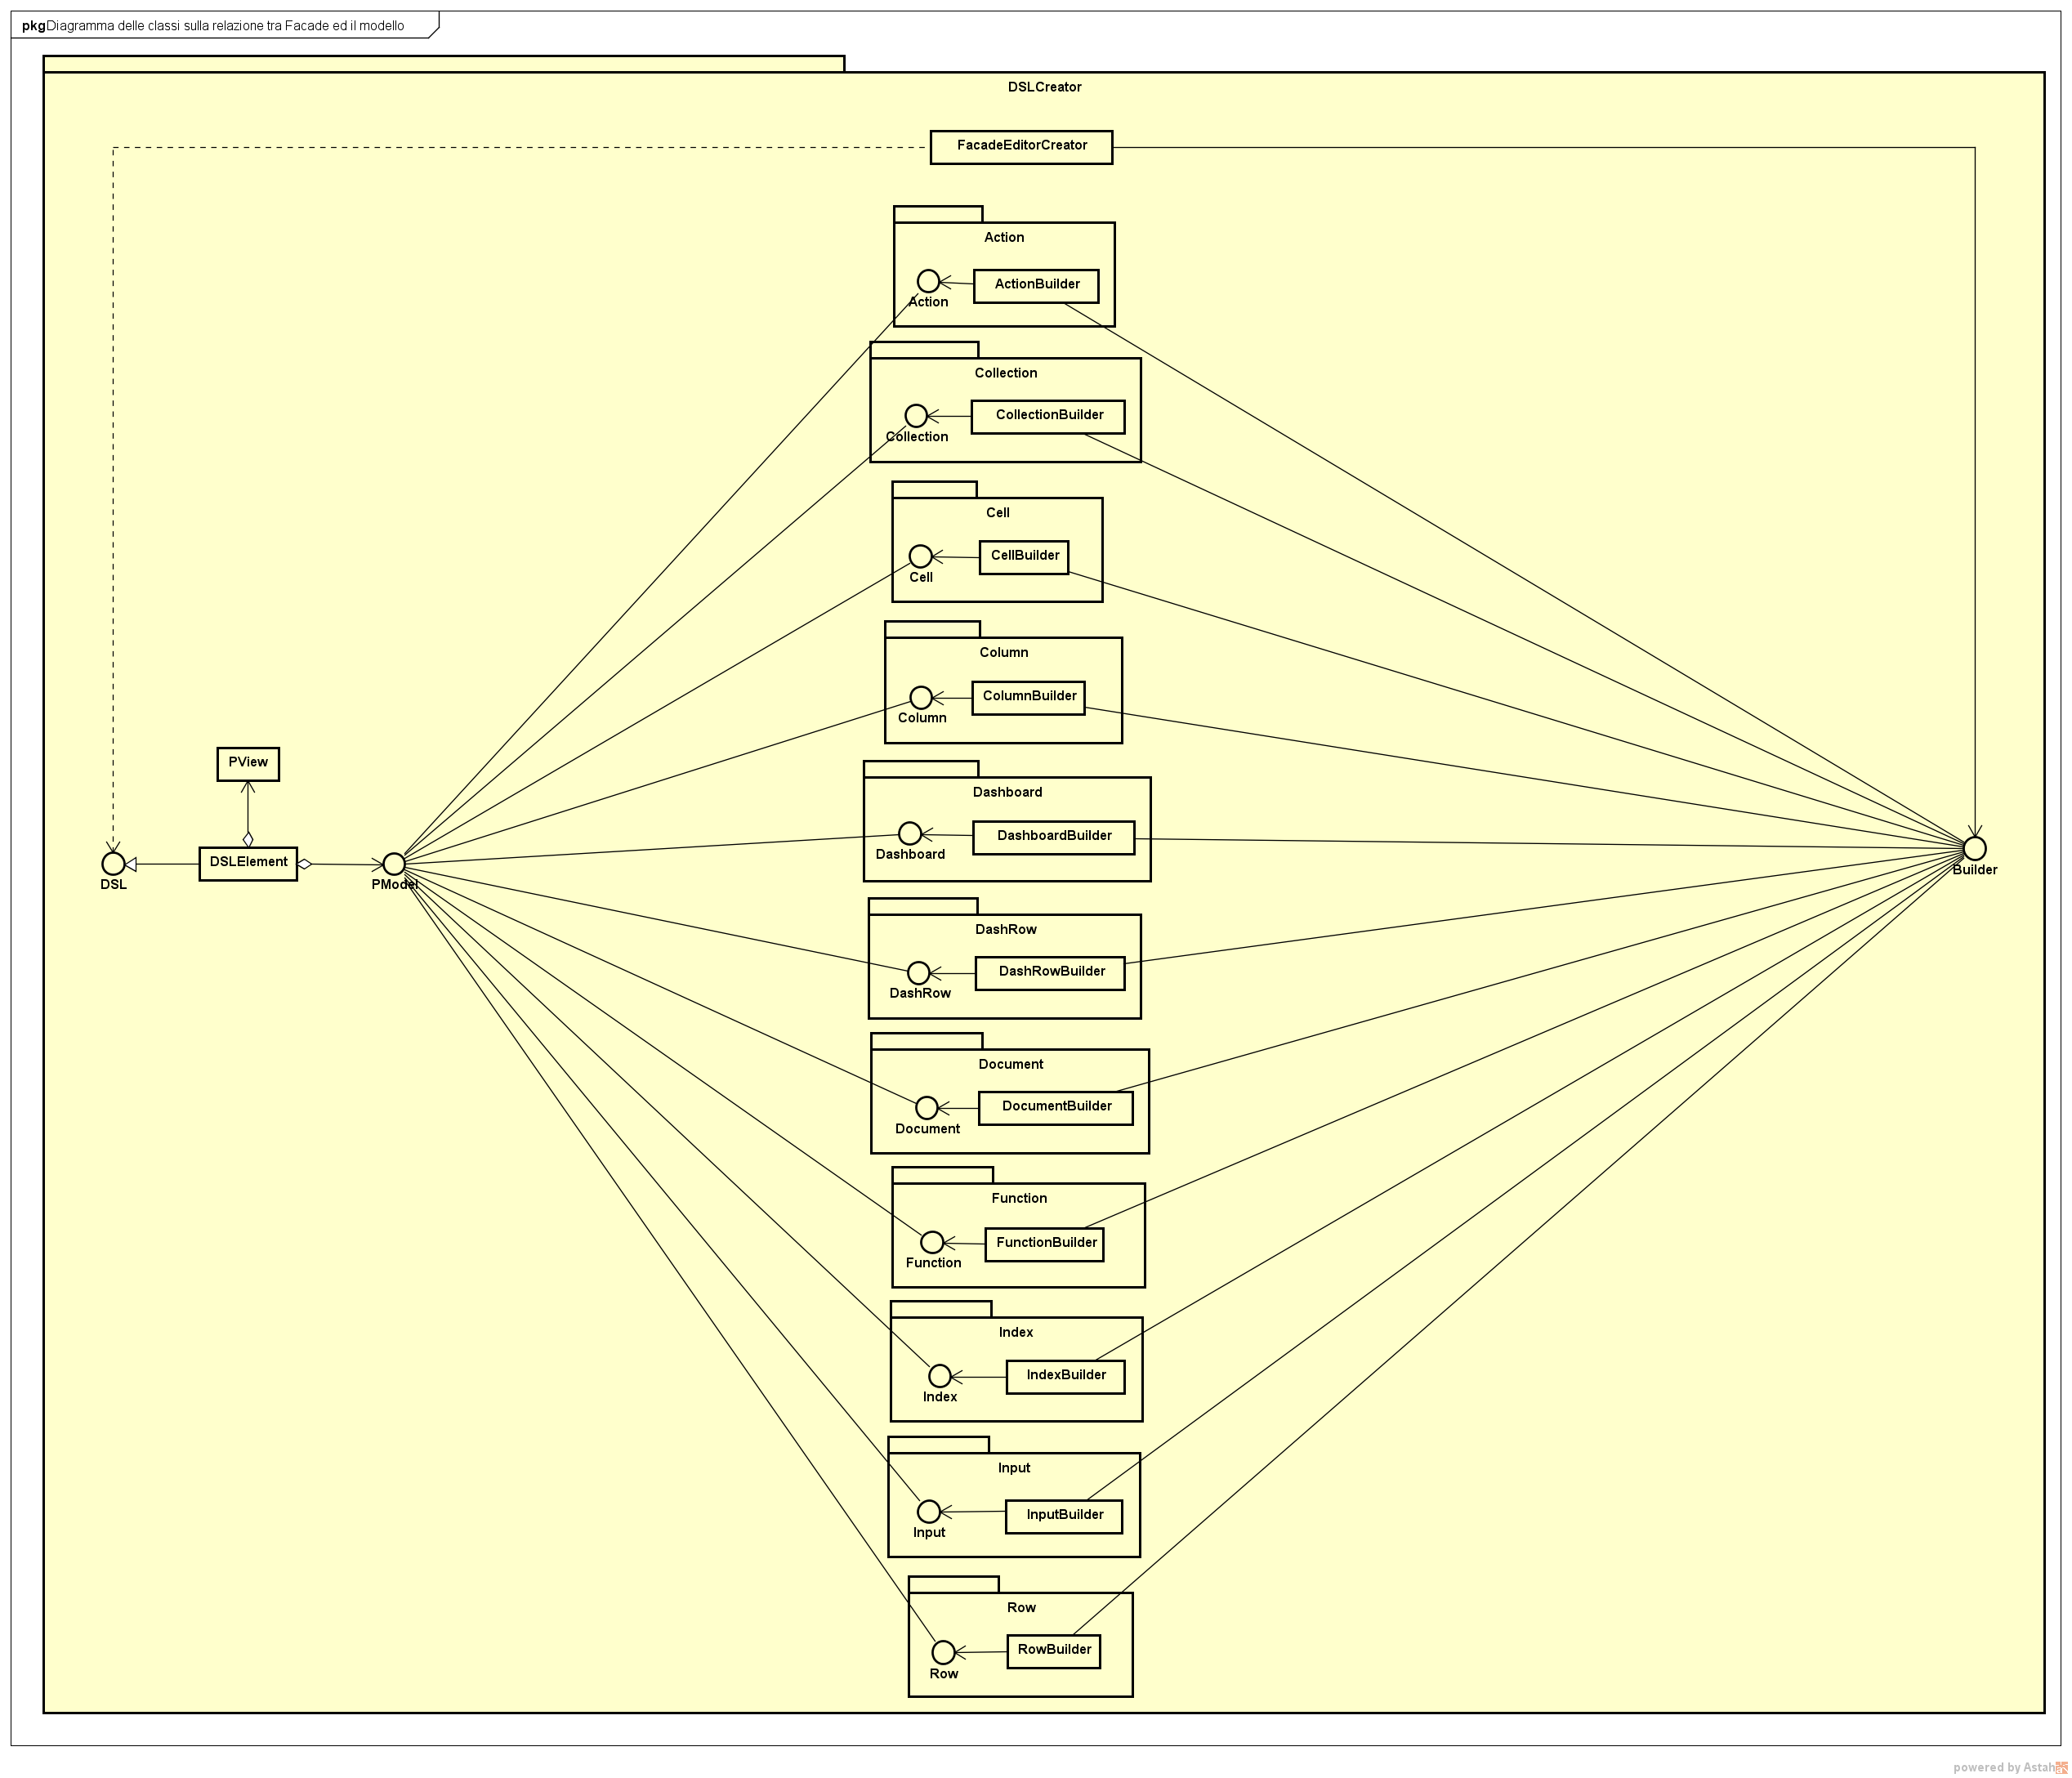
\includegraphics[width=0.9\textwidth]{res/img/diagram_facade.png}
          \caption{Package DSLCreator}
          \label{fig:diagram_model}
        \end{figure}
        \subsubsection{Descrizione}
        In questo \glossaryItem{package} vengono inserite tutte le classi che contribuiscono a creare (e perciò a descrivere) un \glossaryItem{DSL} Element. La classe \glossaryItem{DSL} Element è in relazione di aggregazione con le classi PView e PModel. Queste due classi descrivono aspetti diversi di un \glossaryItem{DSL} Element: la prima ne indica le proprietà grafiche (ad esempio la sua posizione nel piano); la seconda ne descrive il modello (richiesto da \glossaryItem{MaaS}).\\
        Sono stati usati i pattern Facade (in cui le componenti dell'editor rappresentano il sottosistema complesso) e \textit{Builder} (in cui l'oggetto complesso da costruire è rappresentato da PModel).

        \subsubsection{DSLCreator::DSLElement}
        \begin{itemize}
        \item \textbf{Descrizione} \hfill \\
          Questa classe rappresenta un \glossaryItem{DSL} Element. Ha un riferimento a \texttt{DSLCreator::PModel} e \texttt{DSLCreator::PView}.
        \item \textbf{Utilizzo}  \hfill \\
          %viene usata dal Facade nei tipi di ritorno, ha gli stessi metodi
        \item \textbf{Relazioni con altre classi} \hfill 
          \begin{itemize}
          \item DSLCreator::PView. La classe \texttt{DSLCreator::DSLElement} possiede un suo riferimento per memorizzare informazioni grafiche sul DSLElement.
          \item DSLCreator::PModel. La classe \texttt{DSLCreator::DSLElement} possiede un suo riferimento per memorizzare il modello richiesto da MaaS. 
          \item DSLCreator::DSL. La classe \texttt{DSLCreator::DSLElement} implementa i metodi esposti da questa interfaccia, per la gestione di un DSLElement qualsiasi.
          \end{itemize}
        \end{itemize}

        \subsubsection{DSLCreator::PModel}
        \begin{itemize}
        \item \textbf{Descrizione} \hfill \\
          Questa interfaccia rappresenta un modello di \glossaryItem{DSL} (ad esempio, il modello \glossaryItem{DSL} di un \glossaryItem{Collection} Element \`{e} (name: "NomeCollection", label: "CollectionLabel", id: "CollectionId", weight: CollectionWeight)).
        \item \textbf{Utilizzo}  \hfill \\
          Questa interfaccia viene utilizzata da \texttt{DSLCreator::DSLElement} e descrive il modello di \glossaryItem{DSL}.
        \item \textbf{Relazioni con altre classi} \hfill 
          \begin{itemize}
          \item DSLCreator::DSLElement
          \end{itemize}
        \end{itemize}

        \subsubsection{DSLCreator::PView}
        \begin{itemize}
        \item \textbf{Descrizione} \hfill \\
          Questa classe contiene le proprietà grafiche di un \glossaryItem{DSL} Element.
        \item \textbf{Utilizzo}  \hfill \\
          Questa classe viene utilizzata da \texttt{DSLCreator::DSLElement}.
        \item \textbf{Relazioni con altre classi} \hfill 
          \begin{itemize}
          \item DSLCreator::DSLElement
          \end{itemize}
        \end{itemize}

        \subsubsection{DSLCreator::FacadeEditorCreator}
        \begin{itemize}
        \item \textbf{Descrizione} \hfill \\
          Questa classe è la ``Facade'' del Facade Pattern.
        \item \textbf{Utilizzo}  \hfill \\
          Questa classe viene usata per offrire un'interfaccia semplice che consente di costruire i \glossaryItem{DSL} Element.
        \item \textbf{Relazioni con altre classi} \hfill 
          \begin{itemize}
          \item DSLCreator::Builder. Viene usata dalla classe \texttt{DSLCreator::FacadeEditorCreator} per costruire la componente \texttt{DSLCreator::PModel} di un DSLElement.
          \item DSLCreator::DSL. Viene usata dalla classe \texttt{DSLCreator::FacadeEditorCreator} come tipo di ritorno nei metodi di costruzione di un DSLElement.
          \end{itemize}
        \end{itemize}

        \subsubsection{DSLCreator::Builder}
        \begin{itemize}
        \item \textbf{Descrizione} \hfill \\
          Questa è l'interfaccia da cui derivano tutti i \textit{builder} concreti del \glossaryItem{package} \texttt{DSLCreator}.
        \item \textbf{Utilizzo}  \hfill \\
          Questa classe viene utilizzata da \texttt{DSLCreator::Facade} per costruire i \texttt{DSLCreator::PModel} dei \glossaryItem{DSL} Element.
        \item \textbf{Relazioni con altre classi} \hfill 
          \begin{itemize}
          \item DSLCreator::DSLFacade
          \end{itemize}
        \end{itemize}

        \subsection{Modello dell'editor}
        \begin{figure}[H]
          \centering
          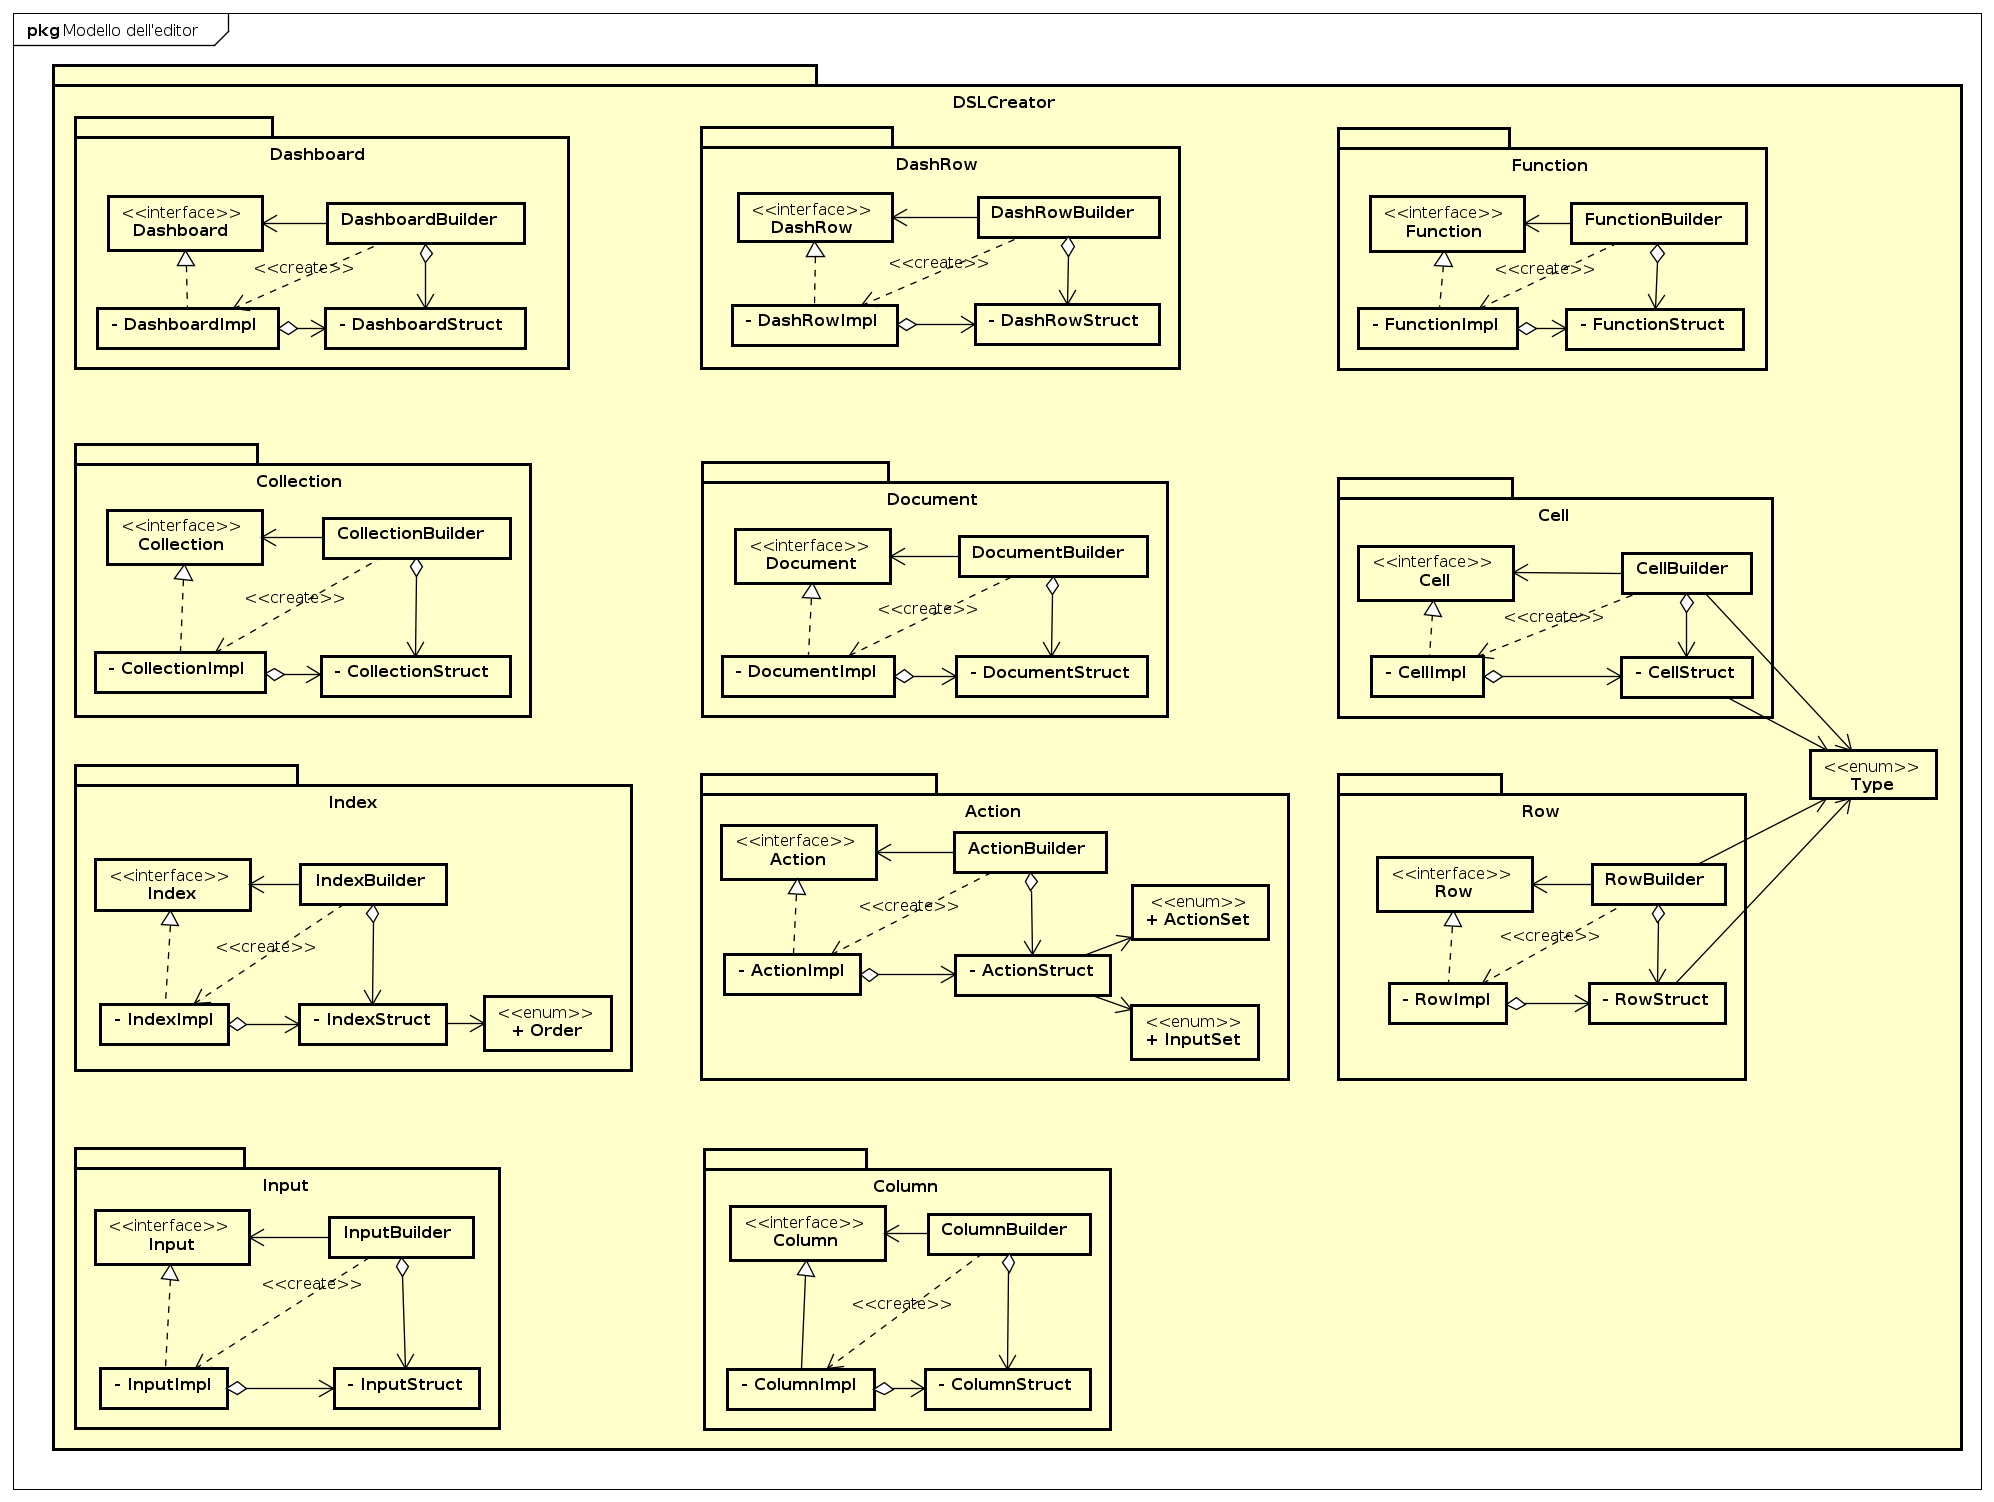
\includegraphics[width=1.1\textwidth]{res/img/Diagram_Model.png}
          \caption{Modello dell'editor}
          \label{fig:diagram_model}
        \end{figure}
        Di seguito, se la classe è visibile all'esterno del rispettivo \glossaryItem{package} non viene scritto nulla, se non lo è verrà specificato.
        \subsection{Package DSLCreator::Dashboard}
                \subsubsection{DSLCreator::Dashboard::Dashboard}
                \begin{figure}[H]
                  \centering
                  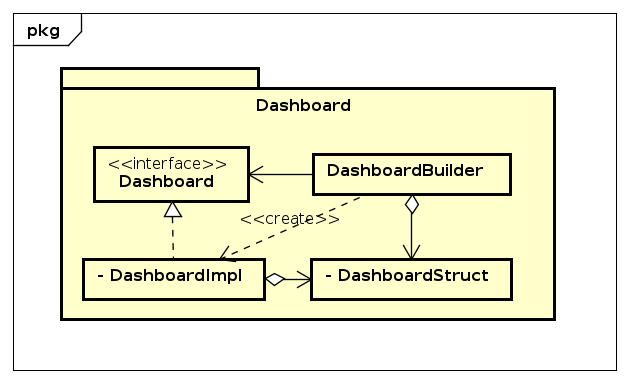
\includegraphics[width=0.7\textwidth]{res/img/Dashboard.png}
                  \caption{Package Dashboard}
                  \label{fig:diagram_model}
                \end{figure}
                    \begin{itemize}
                        \item \textbf{Descrizione} \hfill \\
                            Questa interfaccia rappresenta un \glossaryItem{Dashboard} Element, ossia il ``cruscotto'' che un utente di \glossaryItem{MaaS} può definire (e che verrà visualizzato in forma tabellare nell'applicazione).
                        \item \textbf{Utilizzo}  \hfill \\
                            Questa interfaccia espone le funzionalità di accesso/aggiunta/rimozione a/di \glossaryItem{DashRow Element} (righe della \glossaryItem{Dashboard}), e permette di ottenere/modificare il nome della \glossaryItem{Dashboard}.
                        \item \textbf{Relazioni con altre classi} \hfill 
                            \begin{itemize}
                              \item DSLCreator::Dashboard::DashboardBuilder. Questa classe usa l'interfaccia \texttt{DSLCreator::Dashboard::Dashboard} come tipo di ritorno nel metodo per la costruzione dell'intero prodotto (la dashboard).
                              \item DSLCreator::Dashboard::DashboardImpl. Questa classe implementa i metodi esposti dall'interfaccia \texttt{DSLCreator::Dashboard::Dashboard}.
                            \end{itemize}
                    \end{itemize}

                \subsubsection{DSLCreator::Dashboard::DashboardBuilder}
                    \begin{itemize}
                        \item \textbf{Descrizione} \hfill \\
                            Questa classe costituisce la componente concreta del \textit{Builder} nel \textit{Builder} Pattern.
                        \item \textbf{Utilizzo} \hfill \\
                            Questa classe permette di costruire oggetti \glossaryItem{Dashboard}, di definire un nome e di aggiungere DashRows.
                        \item \textbf{Relazioni con altre classi}
                            \begin{itemize}
                              \item DSLCreator::Dashboard::Dashboard
                              \item DSLCreator::Dashboard::DashboardImpl. Un'istanza di questa classe viene creata da \texttt{DSLCreator::Dashboard::DashboardBuilder}.
                              \item DSLCreator::Dashboard::DashboardStruct. \\ La classe \texttt{DSLCreator::Dashboard::DashboardBuilder} possiede un suo riferimento per memorizzare le informazioni sulla Dashboard che un utente può richiedere di aggiungere (come parti del prodotto da costruire).
                            \end{itemize}
                    \end{itemize}

                \subsubsection{DSLCreator::Dashboard::DashboardImpl}
                    \begin{itemize}
                        \item \textbf{Descrizione} \hfill \\
                            Questa classe implementa l'interfaccia \texttt{DSLCreator::Dashboard::Dashboard} ed ha un costruttore che prende in input un riferimento a un oggetto di tipo \\ \texttt{DSLCreator::Dashboard::DashboardStruct} che contiene le informazioni della \glossaryItem{Dashboard}.
                        \item \textbf{Utilizzo} \hfill \\
                            Questa classe non è visibile all'esterno del \glossaryItem{package} \texttt{DSLCreator::Dashboard} ed una sua istanza viene creata dalla classe \texttt{DSLCreator::Dashboard::DashboardBuilder}.
                        \item \textbf{Relazioni con altre classi}
                            \begin{itemize}
                              \item DSLCreator::Dashboard::Dashboard
                              \item DSLCreator::Dashboard::DashboardBuilder
                              \item DSLCreator::Dashboard::DashboardStruct. \\ La classe \texttt{DSLCreator::Dashboard::DashboardImpl} possiede un suo riferimento, che usa per implementare i metodi esposti dall'interfaccia \texttt{DSLCreator::\-Dashboard::Dashboard}.
                            \end{itemize}
                    \end{itemize}

                \subsubsection{DSLCreator::Dashboard::DashboardStruct}
                    \begin{itemize}
                        \item \textbf{Descrizione} \hfill \\
                            Questa classe contiene le proprietà di una \glossaryItem{Dashboard}: un attributo name (nome della \glossaryItem{Dashboard}) e dei ``riferimenti'' (tramite stringhe) alle DashRow.
                        \item \textbf{Utilizzo} \hfill \\
                            Questa classe non è visibile all'esterno del \glossaryItem{package} \texttt{DSLCreator::Dashboard}. Viene utilizzata da \texttt{DSLCreator::Dashboard::DashboardImpl} e da \texttt{DSLCreator::Dash\-board::DashboardBuilder}: entrambi possiedono un suo riferimento e la usano per memorizzare le proprietà della \glossaryItem{Dashboard}.
                        \item \textbf{Relazioni con altre classi}
                            \begin{itemize}
                              \item DSLCreator::Dashboard::DashboardBuilder
                              \item DSLCreator::Dashboard::DashboardImpl
                            \end{itemize}
                    \end{itemize}
                    
        \subsection{Relazioni fra classi all'interno dei packages}
        Nei packages seguenti, le relazioni tra classi e interfacce sono analoghe a quelle descritte per il package \texttt{DSLCreator::Dashboard}. Esiste in ogni package una classe \textit{builder} che si occupa di costruire il DSLElement e aggiungerne delle proprietà a richiesta. Esiste sempre un'interfaccia, la relativa implementazione e una classe ``struttura'' che contiene le informazioni del DSLElement corrente e che viene usata dal \textit{builder} e dall'implementazione.

        \subsection{Package DSLCreator::DashRow}
                \subsubsection{DSLCreator::DashRow::DashRow}
                \begin{figure}[H]
                  \centering
                  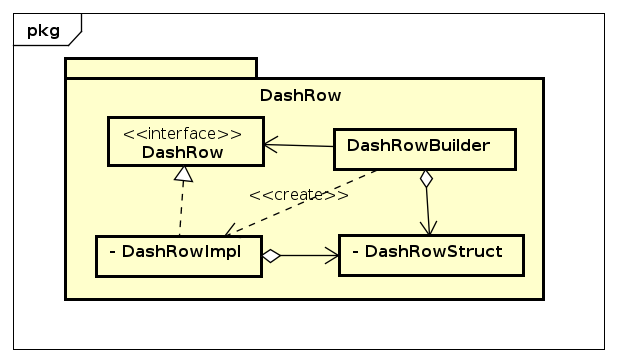
\includegraphics[width=0.7\textwidth]{res/img/DashRow.png}
                  \caption{Package DashRow}
                  \label{fig:diagram_model}
                \end{figure}
                    \begin{itemize}
                        \item \textbf{Descrizione} \hfill \\
                            Questa interfaccia rappresenta un \glossaryItem{DashRow Element}, una riga della \glossaryItem{Dashboard}.
                        \item \textbf{Utilizzo} \hfill \\
                            Questa interfaccia espone delle funzionalità di accesso e di aggiunta/rimozione/modifica di \glossaryItem{DSL} Element in una riga della \glossaryItem{Dashboard}, che possono essere un \glossaryItem{Cell} Element, un \glossaryItem{Document} Element o un \glossaryItem{Collection} Element. 
                        \item \textbf{Relazioni con altre classi}
                            \begin{itemize}
                              \item DSLCreator::DashRow::DashRowBuilder
                              \item DSLCreator::DashRow::DashRowImpl
                            \end{itemize}
                    \end{itemize}

                \subsubsection{DSLCreator::DashRow::DashRowBuilder}
                    \begin{itemize}
                        \item \textbf{Descrizione} \hfill \\
                            Questa classe costituisce la componente concreta del \textit{Builder} nel \textit{Builder} Pattern.
                        \item \textbf{Utilizzo} \hfill \\
                            Questa classe permette di costruire oggetti DashRow e di agganciarci \glossaryItem{Cell} Elements, Documents Elements, \glossaryItem{Collection} Elements.
                        \item \textbf{Relazioni con altre classi}
                            \begin{itemize}
                              \item DSLCreator::DashRow::DashRow
                              \item DSLCreator::DashRow::DashRowImpl
                              \item DSLCreator::DashRow::DashRowStruct
                            \end{itemize}
                    \end{itemize}

 \subsubsection{DSLCreator::DashRow::DashRowImpl}
                    \begin{itemize}
                        \item \textbf{Descrizione} \hfill \\
                            Questa classe implementa l'interfaccia \texttt{DSLCreator::DashRow::DashRow} ed ha un costruttore che prende in input un riferimento ad un oggetto di tipo \texttt{DSLCreator::Dash\-Row::DashRowStruct} che contiene le informazioni della DashRow.
                        \item \textbf{Utilizzo} \hfill \\
                            Questa classe non è visibile all'esterno del \glossaryItem{package} \texttt{DSLCreator::DashRow} ed una sua istanza viene creata dalla classe \texttt{DSLCreator::DashRow::DashRowBuilder}.
                        \item \textbf{Relazioni con altre classi}
                            \begin{itemize}
                              \item DSLCreator::DashRow::DashRow
                              \item DSLCreator::DashRow::DashRowBuilder
                              \item DSLCreator::DashRow::DashRowStruct
                            \end{itemize}
                    \end{itemize}

 \subsubsection{DSLCreator::DashRow::DashRowStruct}
                    \begin{itemize}
                        \item \textbf{Descrizione} \hfill \\
                            Questa classe possiede dei ``riferimenti'' (tramite stringhe) ai \glossaryItem{DSL} Elements che possono essere agganciati ad una \glossaryItem{dashrow}: \glossaryItem{Cell} Element, \glossaryItem{Document} Element o \glossaryItem{Collection} Element.
                        \item \textbf{Utilizzo} \hfill \\
                            Questa classe non è visibile all'esterno del \glossaryItem{package} \texttt{DSLCreator::DashRow}. Viene utilizzata da \texttt{DSLCreator::DashRow::DashRowBuilder} e da \texttt{DSLCreator::Dash\-Row::DashRowImpl}: entrambi possiedono un suo riferimento e la usano per memorizzare le informazioni sui \glossaryItem{DSL} Elements agganciati alla DashRow.
                        \item \textbf{Relazioni con altre classi}
                            \begin{itemize}
                              \item DSLCreator::DashRow::DashRowBuilder
                              \item DSLCreator::DashRow::DashRowImpl
                            \end{itemize}
                    \end{itemize}

\subsection{Package DSLCreator::Collection}
 \subsubsection{DSLCreator::Collection::Collection}
 \begin{figure}[H]
   \centering
   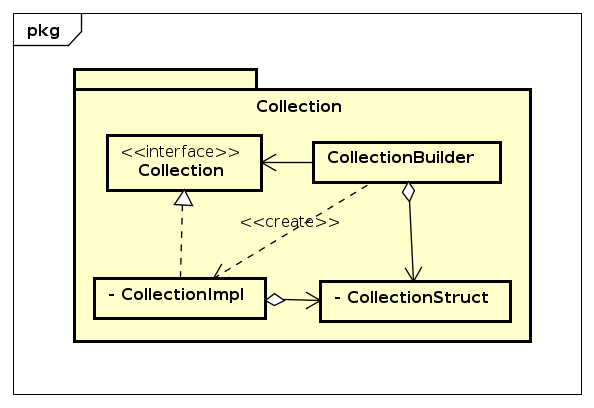
\includegraphics[width=0.7\textwidth]{res/img/Collection.png}
   \caption{Package Collection}
   \label{fig:diagram_model}
 \end{figure}
                    \begin{itemize}
                        \item \textbf{Descrizione} \hfill \\
                            Questa interfaccia rappresenta un \glossaryItem{Collection} Element, ossia una ``collezione'' che può essere inserita in una riga della \glossaryItem{Dashboard}, definita dall'utente di \glossaryItem{MaaS} e che verrà visualizzata in forma tabellare nell'applicazione.
                        \item \textbf{Utilizzo} \hfill \\
                            Questa interfaccia espone le funzionalità per l'accesso e la modifica delle proprietà di una \glossaryItem{Collection}.
                        \item \textbf{Relazioni con altre classi}
                            \begin{itemize}
                              \item DSLCreator::Collection::CollectionBuilder
                              \item DSLCreator::Collection::CollectionImpl
                            \end{itemize}
                    \end{itemize}

 \subsubsection{DSLCreator::Collection::CollectionBuilder}
                    \begin{itemize}
                        \item \textbf{Descrizione} \hfill \\
                            Questa classe costituisce la componente concreta del \textit{Builder} nel \textit{Builder} Pattern.
                        \item \textbf{Utilizzo} \hfill \\
                            Questa classe ha il compito di costruire oggetti \glossaryItem{Collection}, definendone le proprietà.
                        \item \textbf{Relazioni con altre classi}
                            \begin{itemize}
                              \item DSLCreator::Collection::Collection
                              \item DSLCreator::Collection::CollectionImpl
                              \item DSLCreator::Collection::CollectionStruct
                            \end{itemize}
                    \end{itemize}

 \subsubsection{DSLCreator::Collection::CollectionImpl}
                    \begin{itemize}
                        \item \textbf{Descrizione} \hfill \\
                            Questa classe implementa l'interfaccia \texttt{DSLCreator::Collection::Collection} ed è dotata di un costruttore che prende in input un riferimento ad un oggetto di tipo \texttt{DSLCreator::Collection::CollectionStruct}, che contiene le informazioni relative alla \glossaryItem{Collection}.
                        \item \textbf{Utilizzo} \hfill \\
                            Questa classe non è visibile all'esterno del \glossaryItem{package} \texttt{DSLCreator::Collection} ed una sua istanza viene creata dalla classe \texttt{DSLCreator::Collection::CollectionBuilder}.
                        \item \textbf{Relazioni con altre classi}
                            \begin{itemize}
                              \item DSLCreator::Collection::Collection
                              \item DSLCreator::Collection::CollectionBuilder
                              \item DSLCreator::Collection::CollectionStruct
                            \end{itemize}
                    \end{itemize}

 \subsubsection{DSLCreator::Collection::CollectionStruct}
                    \begin{itemize}
                        \item \textbf{Descrizione} \hfill \\
                            Questa classe contiene le proprietà di una \glossaryItem{Collection}: name, label, id, weight, \glossaryItem{index} e \glossaryItem{show}. Possiede dei ``riferimenti'' di tipo stringa ad oggetti di tipo \texttt{DSLCreator::Index::Index}, {DSLCreator::Show::Show} e {DSLCreator::Action::Action} collegati alla \glossaryItem{Collection}.
                        \item \textbf{Utilizzo} \hfill \\
                            Questa classe non è visibile all'esterno del \glossaryItem{package} \texttt{DSLCreator::Collection}. Viene utilizzata dalla classe \texttt{DSLCreator::Collection::CollectionBuilder} e da \texttt{DSLCreator::Collection::CollectionImpl}: entrambe possiedono un suo riferimento e la usano per memorizzare informazioni sulla \glossaryItem{Collection}. 
                        \item \textbf{Relazioni con altre classi}
                            \begin{itemize}
                              \item DSLCreator::Collection::CollectionBuilder
                              \item DSLCreator::Collection::CollectionImpl
                            \end{itemize}
                    \end{itemize}

\subsection{Package DSLCreator::Document}

 \subsubsection{DSLCreator::Document::Document}
                \begin{figure}[H]
                  \centering
                  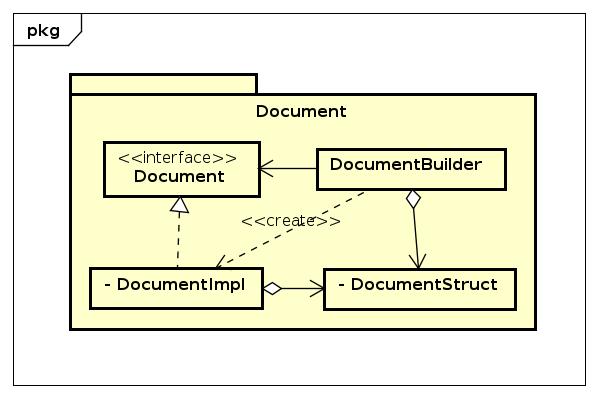
\includegraphics[width=0.7\textwidth]{res/img/Document.png}
                  \caption{Package Document}
                  \label{fig:diagram_model}
                \end{figure}
                    \begin{itemize}
                        \item \textbf{Descrizione} \hfill \\
                            Questa interfaccia rappresenta un \glossaryItem{Document} Element. L'utente può definire un \glossaryItem{Document} e le sue proprietà. Può essere inserito in una riga della \glossaryItem{Dashboard} dell'utente.
                        \item \textbf{Utilizzo} \hfill \\
                            Questa interfaccia espone le funzionalità di accesso e di modifica delle proprietà del \glossaryItem{Document}. Permette l'aggiunta e la rimozione di attributi \glossaryItem{row} (per agganciare un \glossaryItem{Row} Element) e di \glossaryItem{action} (per agganciare un \glossaryItem{Action} Element).
                        \item \textbf{Relazioni con altre classi}
                            \begin{itemize}
                              \item DSLCreator::Document::DocumentBuilder
                              \item DSLCreator::Document::DocumentImpl
                            \end{itemize}
                    \end{itemize}

 \subsubsection{DSLCreator::Document::DocumentBuilder}
                    \begin{itemize}
                        \item \textbf{Descrizione} \hfill \\
                            Questa classe costituisce la componente concreta del \textit{Builder} nel \textit{Builder} Pattern.
                        \item \textbf{Utilizzo} \hfill \\
                            Questa classe ha il compito di costruire oggetti \glossaryItem{Document}, definendone le proprietà.
                        \item \textbf{Relazioni con altre classi}
                            \begin{itemize}
                              \item DSLCreator::Document::Document
                              \item DSLCreator::Document::DocumentImpl
                              \item DSLCreator::Document::DocumentStruct
                            \end{itemize}
                    \end{itemize}

 \subsubsection{DSLCreator::Document::DocumentImpl}
                    \begin{itemize}
                        \item \textbf{Descrizione} \hfill \\
                            Questa classe implementa l'interfaccia \texttt{DSLCreator::Document::DocumentImpl} e ha un costruttore che prende in input un riferimento ad un oggetto di tipo \texttt{DSLCrea\-tor::Document::DocumentStruct}, che contiene le informazioni relative al \glossaryItem{Document}.
                        \item \textbf{Utilizzo} \hfill \\
                            Questa classe non è visibile all'esterno del \glossaryItem{package} \texttt{DSLCreator::Document}. Una sua istanza viene creata dalla classe \texttt{DSLCreator::Document::DocumentBuilder}.
                        \item \textbf{Relazioni con altre classi}
                            \begin{itemize}
                              \item DSLCreator::Document::Document
                              \item DSLCreator::Document::DocumentBuilder
                              \item DSLCreator::Document::DocumentStruct
                            \end{itemize}
                    \end{itemize}

 \subsubsection{DSLCreator::Document::DocumentStruct}
                    \begin{itemize}
                        \item \textbf{Descrizione} \hfill \\
                            Questa classe contiene le proprietà di un \glossaryItem{Document}: l'attributo populate e i ``riferimenti'' di tipo stringa alle \glossaryItem{row} e alle \glossaryItem{Action} agganciate. 
                        \item \textbf{Utilizzo} \hfill \\
                            Questa classe non è visibile all'esterno del \glossaryItem{package} \texttt{DSLCreator::Document}. Viene utilizzata da \texttt{DSLCreator::Document::DocumentBuilder} e da \texttt{DSLCrea\-tor::Document::DocumentImpl}. Entrambe possiedono un suo riferimento e la usano per memorizzare le informazioni sul \glossaryItem{Document}.
                        \item \textbf{Relazioni con altre classi}
                            \begin{itemize}
                              \item DSLCreator::Document::DocumentBuilder
                              \item DSLCreator::Document::DocumentImpl
                            \end{itemize}
                    \end{itemize}

\subsection{Package DSLCreator::Cell}
 \subsubsection{DSLCreator::Cell::Cell}
                 \begin{figure}[H]
                  \centering
                  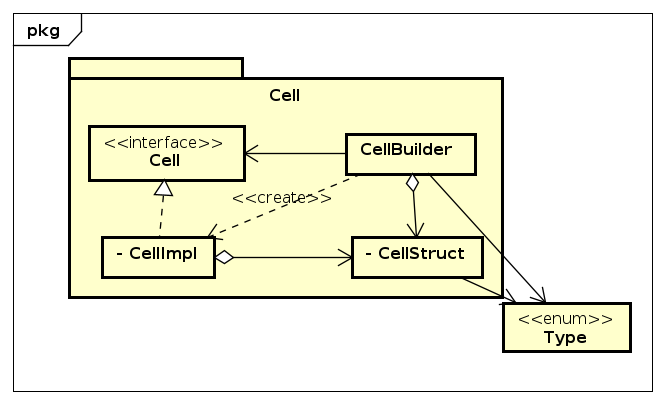
\includegraphics[width=0.7\textwidth]{res/img/Cell.png}
                  \caption{Package Cell}
                  \label{fig:diagram_model}
                \end{figure}
                    \begin{itemize}
                        \item \textbf{Descrizione} \hfill \\
                            Questa interfaccia rappresenta un \glossaryItem{Cell} Element. L'utente può definire il tipo e assegnare un valore che la \glossaryItem{cell} dovrà contenere.
                        \item \textbf{Utilizzo} \hfill \\
                            Questa interfaccia espone le funzionalità per l'accesso e la modifica delle proprietà della \glossaryItem{Cell}.
                        \item \textbf{Relazioni con altre classi}
                            \begin{itemize}
                              \item DSLCreator::Cell::CellBuilder
                              \item DSLCreator::Cell::CellImpl
                            \end{itemize}
                    \end{itemize}

 \subsubsection{DSLCreator::Cell::CellBuilder}
                    \begin{itemize}
                        \item \textbf{Descrizione} \hfill \\
                            Questa classe costituisce la componente concreta del \textit{Builder} nel \textit{Builder} Pattern.
                        \item \textbf{Utilizzo} \hfill \\
                            Questa classe ha il compito di costruire oggetti di tipo \glossaryItem{Cell}, definendone le proprietà.
                        \item \textbf{Relazioni con altre classi}
                            \begin{itemize}
                              \item DSLCreator::Cell::Cell
                              \item DSLCreator::Cell::CellImpl
                              \item DSLCreator::Cell::CellStruct
                              \item DSLCreator::Type
                            \end{itemize}
                    \end{itemize}

 \subsubsection{DSLCreator::Cell::CellImpl}
                    \begin{itemize}
                        \item \textbf{Descrizione} \hfill \\
                            Questa classe implementa l'interfaccia \texttt{DSLCreator::Cell::Cell} e ha un costruttore che prende in input un riferimento ad un oggetto di tipo \texttt{DSLCreator::Cell::CellStruct}, che contiene le informazione della \glossaryItem{cell}.
                        \item \textbf{Utilizzo} \hfill \\
                            Questa classe non è visibile all'esterno del \glossaryItem{package} \texttt{DSLCreator::Cell}. Una sua istanza viene creata dalla classe \texttt{DSLCreator::Cell::CellBuilder}.
                        \item \textbf{Relazioni con altre classi}
                            \begin{itemize}
                              \item DSLCreator::Cell::Cell
                              \item DSLCreator::Cell::CellBuilder
                              \item DSLCreator::Cell::CellStruct
                            \end{itemize}
                    \end{itemize}

 \subsubsection{DSLCreator::Cell::CellStruct}
                    \begin{itemize}
                        \item \textbf{Descrizione} \hfill \\
                            Questa classe contiene le informazioni di una \glossaryItem{Cell} (valore e tipo).
                        \item \textbf{Utilizzo} \hfill \\
                            Questa classe non è visibile all'esterno del \glossaryItem{package} \texttt{DSLCreator::Cell}. Viene utilizzata da \texttt{DSLCreator::Cell::CellBuilder} e \texttt{DSLCreator::Cell::CellImpl}. Entrambe possiedono un suo riferimento e la usano per memorizzare le informazioni relative alla \glossaryItem{Cell}.
                        \item \textbf{Relazioni con altre classi}
                            \begin{itemize}
                              \item DSLCreator::Cell::CellBuilder
                              \item DSLCreator::Cell::CellBuilder
                              \item DSLCreator::Type
                            \end{itemize}
                    \end{itemize}

\subsection{Package DSLCreator::Index}
 \subsubsection{DSLCreator::Index::Index}
                \begin{figure}[H]
                  \centering
                  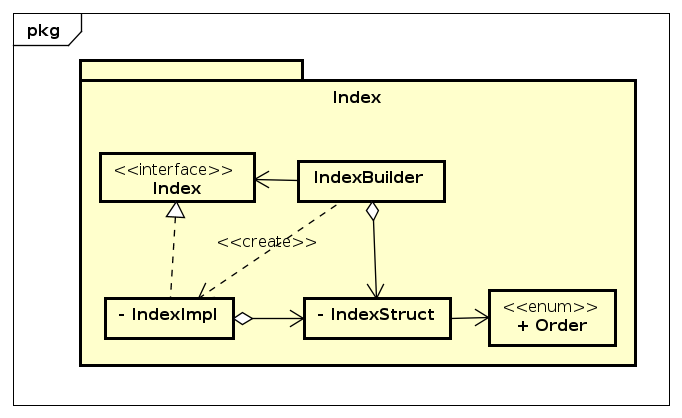
\includegraphics[width=0.7\textwidth]{res/img/Index.png}
                  \caption{Package Index}
                  \label{fig:diagram_model}
                \end{figure}
                    \begin{itemize}
                        \item \textbf{Descrizione} \hfill \\
                            Questa interfaccia rappresenta un \glossaryItem{Index} Element. Specifica come viene configurata una \glossaryItem{Collection} dall'utente. Ad esempio, l'utente può specificare in quale ordine devono essere visualizzati gli elementi nelle righe della \glossaryItem{Collection} e definirne un massimo numero per pagina.
                        \item \textbf{Utilizzo} \hfill \\
                            Questa interfaccia espone le funzionalità di accesso e modifica delle proprietà di \glossaryItem{Index}.
                        \item \textbf{Relazioni con altre classi}
                            \begin{itemize}
                              \item DSLCreator::Index::IndexBuilder
                              \item DSLCreator::Index::IndexStruct
                            \end{itemize}
                    \end{itemize}

 \subsubsection{DSLCreator::Index::IndexBuilder}
                    \begin{itemize}
                        \item \textbf{Descrizione} \hfill \\
                            Questa classe costituisce la componente concreta del \textit{Builder} nel \textit{Builder} Pattern.
                        \item \textbf{Utilizzo} \hfill \\
                            Questa classe ha il compito di creare oggetti \glossaryItem{Index}, definendone le proprietà.
                        \item \textbf{Relazioni con altre classi}
                            \begin{itemize}
                              \item DSLCreator::Index::Index
                              \item DSLCreator::Index::IndexImpl
                              \item DSLCreator::Index::IndexStruct
                            \end{itemize}
                    \end{itemize}
  
 \subsubsection{DSLCreator::Index::IndexImpl}
                    \begin{itemize}
                        \item \textbf{Descrizione} \hfill \\
                          Questa classe implementa l'interfaccia \texttt{DSLCreator::Index::Index} e ha un costruttore che prende in input un riferimento ad un oggetto di tipo \texttt{DSLCrea\-tor::Index::IndexStruct}, che contiene le informazioni relative all'Index.
                        \item \textbf{Utilizzo} \hfill \\
                          Questa classe non è visibile all'esterno del \glossaryItem{package} \texttt{DSLCreator::Index} e una sua istanza può essere creata solo dalla classe \texttt{DSLCreator::Index::IndexBuilder}.
                        \item \textbf{Relazioni con altre classi}
                            \begin{itemize}
                              \item DSLCreator::Index::Index
                              \item DSLCreator::Index::IndexBuilder
                              \item DSLCreator::Index::IndexStruct
                            \end{itemize}
                    \end{itemize}

 \subsubsection{DSLCreator::Index::IndexStruct}
                    \begin{itemize}
                        \item \textbf{Descrizione} \hfill \\
                          Questa classe contiene le informazioni relative a un \glossaryItem{Index} (perpage, populate, sortby, order, query). Contiene inoltre dei ``riferimenti'' di tipo stringa alle \glossaryItem{Column} e agli Input.
                        \item \textbf{Utilizzo} \hfill \\
                          Questa classe non è visibile all'esterno del \glossaryItem{package} \texttt{DSLCreator::Index}. Viene utilizzata da \texttt{DSLCreator::Index::IndexBuilder} e da \texttt{DSLCreator::Index::IndexImpl}. Entrambe possiedono un suo riferimento e la usano per memorizzare le informazioni relative all'Index.
                        \item \textbf{Relazioni con altre classi}
                            \begin{itemize}
                              \item DSLCreator::Index::IndexBuilder
                              \item DSLCreator::Index::IndexImpl
                              \item DSLCreator::Order
                            \end{itemize}
                    \end{itemize}

 \subsubsection{DSLCreator::Index::Order}
                    \begin{itemize}
                        \item \textbf{Descrizione} \hfill \\
                          Questa classe descrive quali valori può avere il campo order di una IndexStruct. 
                        \item \textbf{Utilizzo} \hfill \\
                          Questa classe viene utilizzata da una IndexStruct per definire l'ordinamento (crescente o decrescente) degli elementi nelle righe di una \glossaryItem{Collection}.
                        \item \textbf{Relazioni con altre classi}
                            \begin{itemize}
                              \item DSLCreator::Index::IndexStruct
                            \end{itemize}
                    \end{itemize}

\subsection{Package DSLCreator::Row}
 \subsubsection{DSLCreator::Row::Row}
                 \begin{figure}[H]
                  \centering
                  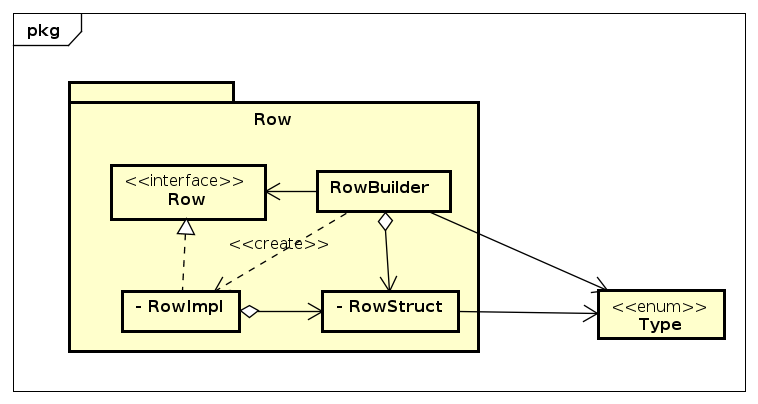
\includegraphics[width=0.7\textwidth]{res/img/Row.png}
                  \caption{Package Row}
                  \label{fig:diagram_model}
                \end{figure}
                    \begin{itemize}
                        \item \textbf{Descrizione} \hfill \\
                          Questa interfaccia rappresenta un \glossaryItem{Row} Element. Specifica come viene configurata una riga di un \glossaryItem{Document} dall'utente.
                        \item \textbf{Utilizzo} \hfill \\
                          Questa interfaccia espone le funzionalità di accesso/modifica delle proprietà di una \glossaryItem{Row}.
                        \item \textbf{Relazioni con altre classi}
                            \begin{itemize}
                              \item DSLCreator::Row::RowBuilder
                              \item DSLCreator::Row::RowImpl
                            \end{itemize}
                    \end{itemize}

 \subsubsection{DSLCreator::Row::RowBuilder}
                    \begin{itemize}
                        \item \textbf{Descrizione} \hfill \\
                          Questa classe costituisce la componente concreta del \textit{Builder} nel \textit{Builder} Pattern.
                        \item \textbf{Utilizzo} \hfill \\
                          Questa classe viene usata per costruire oggetti \glossaryItem{Row} e settarne le proprietà.
                        \item \textbf{Relazioni con altre classi}
                            \begin{itemize}
                              \item DSLCreator::Row::Row
                              \item DSLCreator::Row::RowImpl
                              \item DSLCreator::Row::RowStruct
                              \item DSLCreator::Type
                            \end{itemize}
                    \end{itemize}  

 \subsubsection{DSLCreator::Row::RowImpl}
                    \begin{itemize}
                        \item \textbf{Descrizione} \hfill \\
                          Questa classe implementa l'interfaccia \texttt{DSLCreator::Row::Row} e ha un costruttore che prende in input un riferimento ad un oggetto di tipo \texttt{DSLCreator::Row::RowStruct}, che contiene le informazioni sulla \glossaryItem{Row}.
                        \item \textbf{Utilizzo} \hfill \\
                          Questa classe non è visibile all'esterno del \glossaryItem{package} \texttt{DSLCreator::Row} ed una sua istanza viene creata dalla classe \texttt{DSLCreator::Row::RowBuilder}.
                        \item \textbf{Relazioni con altre classi}
                            \begin{itemize}
                              \item DSLCreator::Row::Row
                              \item DSLCreator::Row::RowBuilder
                              \item DSLCreator::Row::RowStruct
                            \end{itemize}
                    \end{itemize}  

 \subsubsection{DSLCreator::Row::RowStruct}
                    \begin{itemize}
                        \item \textbf{Descrizione} \hfill \\
                          Questa classe contiene le proprietà di una \glossaryItem{Row} (name, label, transformation, type).
                        \item \textbf{Utilizzo} \hfill \\
                          Questa classe non è visibile all'esterno del \glossaryItem{package} \texttt{DSLCreator::Row}. Viene utilizzata da \texttt{DSLCreator::Row::RowBuilder} e da \texttt{DSLCreator::Row::RowImpl}. Entrambe possiedono un suo riferimento e la usano per memorizzare le informazioni di una \glossaryItem{row}.
                        \item \textbf{Relazioni con altre classi}
                            \begin{itemize}
                              \item DSLCreator::Row::RowBuilder
                              \item DSLCreator::Row::RowImpl
                              \item DSLCreator::Type
                            \end{itemize}
                    \end{itemize}  

\subsection{Package DSLCreator::Column}
 \subsubsection{DSLCreator::Column::Column}
                 \begin{figure}[H]
                  \centering
                  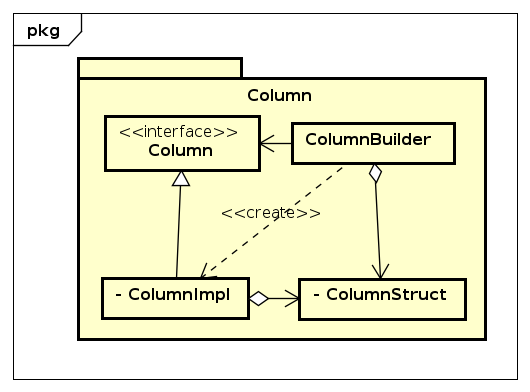
\includegraphics[width=0.7\textwidth]{res/img/Column.png}
                  \caption{Package Column}
                  \label{fig:diagram_model}
                \end{figure}
                    \begin{itemize}
                        \item \textbf{Descrizione} \hfill \\
                          Questa interfaccia rappresenta un \glossaryItem{Column} Element. Specifica come viene configurata una colonna di una \glossaryItem{Collection} dall'utente. Ad esempio, l'utente può rendere una colonna ordinabile oppure no.
                        \item \textbf{Utilizzo} \hfill \\
                          Questa interfaccia espone le funzionalità di accesso e modifica delle proprietà di una \glossaryItem{Column}.
                        \item \textbf{Relazioni con altre classi}
                            \begin{itemize}
                              \item DSLCreator::Column::ColumnBuilder
                              \item DSLCreator::Column::ColumnImpl
                            \end{itemize}
                    \end{itemize}  

 \subsubsection{DSLCreator::ColumnBuilder}
                    \begin{itemize}
                        \item \textbf{Descrizione} \hfill \\
                          Questa classe costituisce la componente concreta del \textit{Builder} nel \textit{Builder} Pattern.
                        \item \textbf{Utilizzo} \hfill \\
                          Questa classe ha il compito di costruire oggetti \glossaryItem{Column} e di definirne le proprietà.
                        \item \textbf{Relazioni con altre classi}
                            \begin{itemize}
                              \item DSLCreator::Column::Column
                              \item DSLCreator::Column::ColumnImpl
                              \item DSLCreator::Column::ColumnStruct
                            \end{itemize}
                    \end{itemize}  

 \subsubsection{DSLCreator::Column::ColumnImpl}
                    \begin{itemize}
                        \item \textbf{Descrizione} \hfill \\
                          Questa classe implementa l'interfaccia \texttt{DSLCreator::Column::Column} ed ha un costruttore che prende in input un riferimento ad un oggetto di tipo \texttt{DSLCreator::Co\-lumn::ColumnStruct}, che contiene le informazioni sulla \glossaryItem{Column}.
                        \item \textbf{Utilizzo} \hfill \\
                          Questa classe non è visibile all'esterno del \glossaryItem{package} \texttt{DSLCreator::Column} ed una sua istanza viene creata dalla classe \texttt{DSLCreator::Column::ColumnBuilder}.
                        \item \textbf{Relazioni con altre classi}
                            \begin{itemize}
                              \item DSLCreator::Column::Column
                              \item DSLCreator::Column::ColumnBuilder
                              \item DSLCreator::Column::ColumnStruct
                            \end{itemize}
                    \end{itemize}  

 \subsubsection{DSLCreator::ColumnStruct}
                    \begin{itemize}
                        \item \textbf{Descrizione} \hfill \\
                          Questa classe contiene le proprietà di una \glossaryItem{Column} (name, label, sortable, selectable, transformation).
                        \item \textbf{Utilizzo} \hfill \\
                          Questa classe non è visibile all'esterno del \glossaryItem{package} \texttt{DSLCreator::Column}. Viene utilizzata da \texttt{DSLCreator::Column::ColumnBuilder} e da \texttt{DSLCreator::Column::ColumnImpl} ed entrambe possiedono un suo riferimento, che usano per memorizzare le informazioni di una \glossaryItem{Column}.
                        \item \textbf{Relazioni con altre classi}
                            \begin{itemize}
                              \item DSLCreator::Column::ColumnBuilder
                              \item DSLCreator::Column::ColumnImpl
                            \end{itemize}
                    \end{itemize}  

\subsection{Package DSLCreator::Action}
 \subsubsection{DSLCreator::Action::Action}
                 \begin{figure}[H]
                  \centering
                  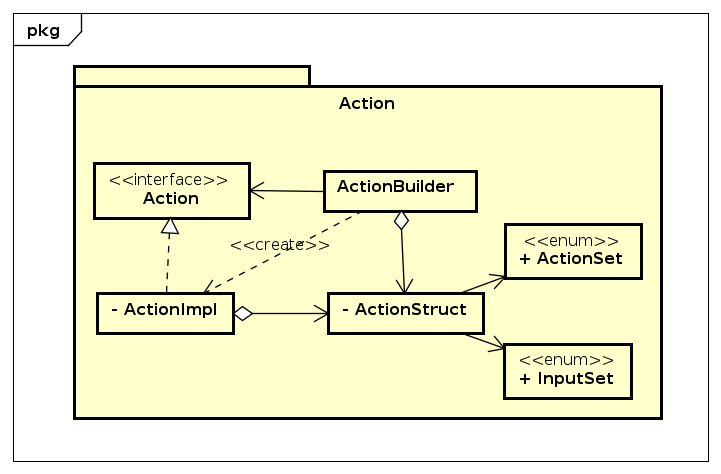
\includegraphics[width=0.7\textwidth]{res/img/Action.png}
                  \caption{Package Action}
                  \label{fig:diagram_model}
                \end{figure}
                    \begin{itemize}
                        \item \textbf{Descrizione} \hfill \\
                          Questa interfaccia rappresenta un \glossaryItem{Action} Element. Specifica quale azione l'utente può agganciare ad un \glossaryItem{Document} o ad una \glossaryItem{Collection}. Ad esempio, l'utente può specificare che tipo di azione desidera (export o send mail) e, nel caso la applichi ad una \glossaryItem{Collection}, quale insieme avrà in input (tutta la \glossaryItem{collection} o solamente quello correntemente visualizzato).
                        \item \textbf{Utilizzo} \hfill \\
                          Questa interfaccia espone le funzionalità di accesso e modifica delle proprietà della \glossaryItem{Action}.
                        \item \textbf{Relazioni con altre classi}
                            \begin{itemize}
                              \item DSLCreator::Action::ActionImpl
                              \item DSLCreator::Action::ActionBuilder
                            \end{itemize}
                    \end{itemize}  

 \subsubsection{DSLCreator::Action::ActionBuilder}
                    \begin{itemize}
                        \item \textbf{Descrizione} \hfill \\
                          Questa classe costituisce la componente concreta del \textit{Builder} nel \textit{Builder} Pattern.
                        \item \textbf{Utilizzo} \hfill \\
                          Questa classe ha il compito di costruire oggetti di tipo \glossaryItem{Action} e di definirne le proprietà.
                        \item \textbf{Relazioni con altre classi}
                            \begin{itemize}
                              \item DSLCreator::Action::Action
                              \item DSLCreator::Action::ActionImpl
                              \item DSLCreator::Action::ActionStruct
                            \end{itemize}
                    \end{itemize}  

 \subsubsection{DSLCreator::Action::ActionImpl}
                    \begin{itemize}
                        \item \textbf{Descrizione} \hfill \\
                          Questa classe implementa l'interfaccia \texttt{DSLCreator::Action::Action} ed ha un costruttore che prende in input un riferimento ad un oggetto di tipo \texttt{DSLCrea\-tor::Action::ActionStruct}, che contiene le informazione dell'Action.
                        \item \textbf{Utilizzo} \hfill \\
                          Questa classe non è visibile all'esterno del \glossaryItem{package} \texttt{DSLCreator::Action} ed una sua istanza viene costruita dalla classe \texttt{DSLCreator::Action::ActionBuilder}.
                        \item \textbf{Relazioni con altre classi}
                            \begin{itemize}
                              \item DSLCreator::Action::Action
                              \item DSLCreator::Action::ActionBuilder
                              \item DSLCreator::Action::ActionStruct
                            \end{itemize}
                    \end{itemize}  

 \subsubsection{DSLCreator::Action::ActionStruct}
                    \begin{itemize}
                        \item \textbf{Descrizione} \hfill \\
                          Questa classe contiene le informazioni di una \glossaryItem{Action} (type, set).
                        \item \textbf{Utilizzo} \hfill \\
                          Questa classe non è visibile all'esterno del \glossaryItem{package} \texttt{DSLCreator::Action}. Viene utilizzata da \texttt{DSLCreator::Action::ActionBuilder} e da \texttt{DSLCrea\-tor::Action::ActionImpl} per memorizzare le informazioni relative all'Action.
                        \item \textbf{Relazioni con altre classi}
                            \begin{itemize}
                              \item DSLCreator::Action::ActionBuilder
                              \item DSLCreator::Action::ActionImpl
                              \item DSLCreator::Action::InputSet
                              \item DSLCreator::Action::ActionSet
                            \end{itemize}
                    \end{itemize}  

 \subsubsection{DSLCreator::Action::InputSet}
                    \begin{itemize}
                        \item \textbf{Descrizione} \hfill \\
                          Questa classe rappresenta il sottoinsieme di una \glossaryItem{Collection} a cui si desidera applicare un'azione.
                        \item \textbf{Utilizzo} \hfill \\
                          Questa classe viene usata per specificare quale sottoinsieme di una \glossaryItem{Collection} dare in input a una \glossaryItem{Action} (due opzioni disponibili: ``whole'' oppure ``visualized'').
                        \item \textbf{Relazioni con altre classi}
                            \begin{itemize}
                              \item DSLCreator::Action::ActionStruct
                            \end{itemize}
                    \end{itemize}  

 \subsubsection{DSLCreator::Action::ActionSet}
                    \begin{itemize}
                        \item \textbf{Descrizione} \hfill \\
                          Questa classe rappresenta i due tipi di azione (export, send mail) che un utente può agganciare ad un \glossaryItem{Document} o ad una \glossaryItem{Collection}.
                        \item \textbf{Utilizzo} \hfill \\
                          Questa classe viene usata per specificare il tipo di azione applicata ad un \glossaryItem{Document} o ad una \glossaryItem{Collection}.
                        \item \textbf{Relazioni con altre classi}
                            \begin{itemize}
                              \item DSLCreator::Action::ActionStruct
                            \end{itemize}
                    \end{itemize}  

\subsection{Package DSLCreator::Input}
 \subsubsection{DSLCreator::Input::Input}
                 \begin{figure}[H]
                  \centering
                  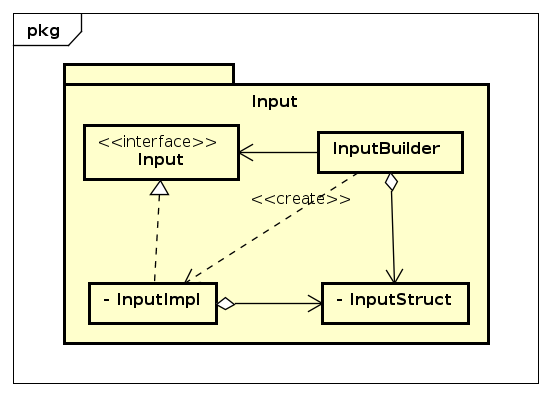
\includegraphics[width=0.7\textwidth]{res/img/Input.png}
                  \caption{Package Input}
                  \label{fig:diagram_model}
                \end{figure}
                    \begin{itemize}
                        \item \textbf{Descrizione} \hfill \\
                          Questa interfaccia rappresenta un \glossaryItem{Input Element}.
                        \item \textbf{Utilizzo} \hfill \\
                          Questa interfaccia espone le funzionalità di accesso e modifica alle proprietà di un \glossaryItem{Input Element} e di aggiunta e rimozione di altri Input ad esso collegati.
                        \item \textbf{Relazioni con altre classi}
                            \begin{itemize}
                              \item DSLCreator::Input::InputBuilder
                              \item DSLCreator::Input::InputImpl
                              \item DSLCreator::Input::InputStruct
                            \end{itemize}
                    \end{itemize}  

 \subsubsection{DSLCreator::Input::InputBuilder}
                    \begin{itemize}
                        \item \textbf{Descrizione} \hfill \\
                          Questa classe costituisce la componente concreta del \textit{Builder} nel \textit{Builder} Pattern.
                        \item \textbf{Utilizzo} \hfill \\
                          Questa classe ha il compito di costruire oggetti Input e di agganciare all'oggetto in costruzione altri oggetti Input o altre proprietà (coppia chiave-valore).
                        \item \textbf{Relazioni con altre classi}
                            \begin{itemize}
                              \item DSLCreator::Input::Input
                              \item DSLCreator::Input::InputImpl
                              \item DSLCreator::Input::InputStruct
                            \end{itemize}
                    \end{itemize}  

 \subsubsection{DSLCreator::Input::InputImpl}
                    \begin{itemize}
                        \item \textbf{Descrizione} \hfill \\
                          Questa classe implementa l'interfaccia \texttt{DSLCreator::Input::Input} ed ha un costruttore che prende in input un riferimento ad un oggetto di tipo \texttt{DSLCrea\-tor::Input::InputStruct}, che contiene le informazioni dell'Input.
                        \item \textbf{Utilizzo} \hfill \\
                          Questa classe non è visibile all'esterno del \glossaryItem{package} \texttt{DSLCreator::Input}. Una sua istanza viene costruita dalla classe \texttt{DSLCreator::Input::InputBuilder}.
                        \item \textbf{Relazioni con altre classi}
                            \begin{itemize}
                              \item DSLCreator::Input::Input
                              \item DSLCreator::Input::InputBuilder
                              \item DSLCreator::Input::InputStruct
                            \end{itemize}
                    \end{itemize}  

 \subsubsection{DSLCreator::Input::InputStruct}
                    \begin{itemize}
                        \item \textbf{Descrizione} \hfill \\
                          Questa classe contiene le proprietà di un Input, ossia due mappe che mantengono le associazioni tra chiavi/valori e tra chiavi/Input.
                        \item \textbf{Utilizzo} \hfill \\
                          Questa classe non è visibile all'esterno del \glossaryItem{package} \texttt{DSLCreator::Input}. Viene utilizzata da \texttt{DSLCreator::Input::InputBuilder} e da \texttt{DSLCreator::Input::InputImpl} per memorizzare le informazioni dell'Input.
                        \item \textbf{Relazioni con altre classi}
                            \begin{itemize}
                              \item DSLCreator::Input::InputImpl
                              \item DSLCreator::Input::InputStruct
                            \end{itemize}
                    \end{itemize}  

\subsection{Package DSLCreator::Function}
 \subsubsection{DSLCreator::Function::Function}
                 \begin{figure}[H]
                  \centering
                  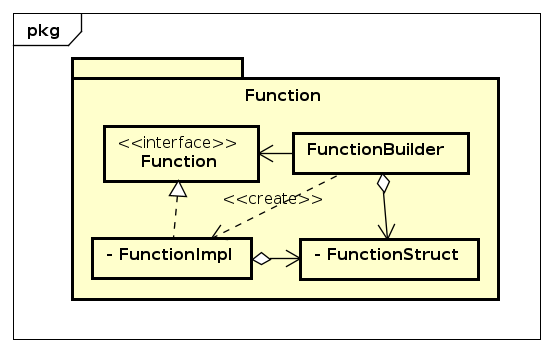
\includegraphics[width=0.7\textwidth]{res/img/Function.png}
                  \caption{Package Function}
                  \label{fig:diagram_model}
                \end{figure}
                    \begin{itemize}
                        \item \textbf{Descrizione} \hfill \\
                          Questa interfaccia rappresenta un \glossaryItem{Function Element}. 
                        \item \textbf{Utilizzo} \hfill \\
                          Questa interfaccia espone le funzionalità di accesso e modifica della proprietà di una Function.
                        \item \textbf{Relazioni con altre classi}
                            \begin{itemize}
                              \item DSLCreator::Function::FunctionBuilder
                              \item DSLCreator::Function::FunctionImpl
                            \end{itemize}
                    \end{itemize}  

 \subsubsection{DSLCreator::Function::FunctionBuilder}
                    \begin{itemize}
                        \item \textbf{Descrizione} \hfill \\
                          Questa classe costituisce la componente concreta del \textit{Builder} nel \textit{Builder} Pattern.
                        \item \textbf{Utilizzo} \hfill \\
                          Questa classe ha il compito di costruire oggetti di tipo Function, definendone le proprietà.
                        \item \textbf{Relazioni con altre classi}
                            \begin{itemize}
                              \item DSLCreator::Function::Function
                              \item DSLCreator::Function::FunctionImpl
                              \item DSLCreator::Function::FunctionStruct
                            \end{itemize}
                    \end{itemize}  

 \subsubsection{DSLCreator::Function::FunctionImpl}
                    \begin{itemize}
                        \item \textbf{Descrizione} \hfill \\
                          Questa classe implementa l'interfaccia \texttt{DSLCreator::Function::Function}; possiede un costruttore che prende in input un riferimento ad un oggetto di tipo \texttt{DSLCreator::Function::FunctionStruct}, che contiene le informazioni della Function.
                        \item \textbf{Utilizzo} \hfill \\
                          Questa classe non è visibile all'esterno del \glossaryItem{package} \texttt{DSLCreator::Function} e una sua istanza viene creata dalla classe \texttt{DSLCreator::Function::FunctionBuilder}.
                        \item \textbf{Relazioni con altre classi}
                            \begin{itemize}
                              \item DSLCreator::Function::Function
                              \item DSLCreator::Function::FunctionBuilder
                              \item DSLCreator::Function::FunctionStruct
                            \end{itemize}
                    \end{itemize}  

 \subsubsection{DSLCreator::Function::FunctionStruct}
                    \begin{itemize}
                        \item \textbf{Descrizione} \hfill \\
                          Questa classe contiene le proprietà di una Function (input, output e definition).
                        \item \textbf{Utilizzo} \hfill \\
                          Questa classe non è visibile all'esterno del \glossaryItem{package} \texttt{DSLCreator::Function::FunctionStruct} ed è utilizzata da \texttt{DSLCreator::Function::FunctionBuilder} e da \texttt{DSLCreator::Fun\-ction::FunctionImpl} per memorizzare le informazioni della Function.
                        \item \textbf{Relazioni con altre classi}
                            \begin{itemize}
                              \item DSLCreator::Function::FunctionBuilder
                              \item DSLCreator::Function::FunctionImpl
                            \end{itemize}
                    \end{itemize}  
